\documentclass[11pt,aspectratio=169]{beamer}

% my packages and definitions
\usepackage{tikz}
\usepackage[font=scriptsize,labelformat=empty]{caption}

\usetikzlibrary{automata, positioning,shapes,arrows}
\usetikzlibrary{fit}
\usepackage[normalem]{ulem}
\newcommand\redout{\bgroup\markoverwith
{\textcolor{red}{\rule[.5ex]{2pt}{0.4pt}}}\ULon}
\usepackage{xcolor}

\usepackage{tcolorbox}
\tcbuselibrary{theorems}

\DeclareMathOperator{\tr}{tr}
\newcommand{\norm}[1]{\left\lVert#1\right\rVert}
\newcommand{\R}{\mathbb{R}}
\newcommand{\dd}{\mathrm{d}}
\newcommand{\myvec}[1]{\ensuremath{\begin{pmatrix}#1\end{pmatrix}}}
\newcommand*{\V}[1]{\mathbf{#1}}
\newcommand{\E}{\mathbb{E}}
\DeclareMathOperator*{\argmin}{\arg\!\min}
\DeclareMathOperator*{\argmax}{\arg\!\max}

\title{Delayed deep learning for continuous-time dynamical systems}
\date[03.03.21]{Master thesis presentation\\Supervising Professors: Prof. Andreas Krause, Prof. Florian Dörfler\\
Supervisor: Philippe Wenk}
\author{Andreas Schlaginhaufen}
\institute{D-INFK \& D-ITET}

\usetheme{eth}

\colorlet{titlefgcolor}{ETH3}
\colorlet{accentcolor}{ETH7}

\begin{document}

%\def\titlefigure{elements/title-page-image}		% Default image
%\def\titlefigure{elements/title-page-image-43}	% Use this for 4:3 presentations
\colorlet{titlefgcolor}{ETH4}
\colorlet{titlebgcolor}{ETH2}
\def\titlefigure{}
\setlength{\titleboxwidth}{0.75\textwidth}			% Change box width
\titleframe

% \colorlet{titlefgcolor}{ETH5}
% \def\titlefigure{elements/title-page-image-alt}
% \title{Different background}
% \titleframe

% \colorlet{titlefgcolor}{ETH4}
% \colorlet{titlebgcolor}{ETH2}
% \def\titlefigure{}
% \setlength{\titleboxwidth}{0.75\textwidth}			% Change box width
% \title{Delayed deep learning for continuous-time dynamical systems}
% \titleframe

%%%%%%%%%%%%%%%%%%%%%%%%%%%%%%%%%%%%%%%%%%%%%%%%%%%%
% 1 Motivation
%%%%%%%%%%%%%%%%%%%%%%%%%%%%%%%%%%%%%%%%%%%%%%%%%%%%

\begin{frame}[t]
    \frametitle{Motivation}
    \textbf{Neural ODE:} \hspace{1cm}\raisebox{-0.2cm}{\begin{tikzpicture}[minimum size=0.6cm, line width=0.75pt]  
        \node[] (x) {$x(t)$};
        \node[rectangle, draw, right=of x] (nn) {NN};
        \node[right=of nn] (dx) {$\dot{x}(t)$};
        \draw[every loop]
        (x) edge[] node {} (nn)
        (nn) edge[] node {} (dx);
    \end{tikzpicture}}\\\vspace{0.2cm}
    \pause
    \textbf{Problem:}\; $\dot{x}(t) = f(x(t))$ is Markovian!
    \begin{itemize}
        \pause
        \vspace{0.2cm}
        \item Discrete-time
            \begin{flalign*}
            &\Delta x_{t+1} = f(\underbrace{x_t, x_{t-1}, ..., x_{t-K}}_{\textcolor{blue}{z_t}},\theta)&
            \end{flalign*}
            \begin{picture}(50,50) \put(330,80){\hbox{\begin{tikzpicture}[overlay, line width=0.75pt]
                \node[state, draw, text width=0.6cm, text centered] (t+1)  {$x_{t+1}$};
                \node[state, draw,left=of t+1, text width=0.6cm, text centered] (t)  {$x_{t}$};
                \node[state, draw,left=of t, text width=0.6cm, text centered] (t-1)  {$x_{t-K}$};
                \path (t) -- node[auto=false]{\ldots} (t-1);
                \draw[every loop]
                (t) edge[] node {} (t+1)
                (t-1) edge[bend left] node {} (t+1);
                \node[ellipse, draw=blue,dotted,label=below:$\textcolor{blue}{z_t}$, fit=(t-1) (t)] {};
            \end{tikzpicture}}} \end{picture}
        \pause
        \vspace{-1cm}
        \item Continuous-time?
            \begin{flalign*}
            &\dot{x}(t) = f(\textcolor{red}{x_t}), \quad x_t(s) := x(t+s),\quad s \in [-r, 0]\quad &\\
            &\;\text{\textcolor{red}{$\to\; x_t$ is $\infty$-dimensional}}&
            \end{flalign*}
        \end{itemize}
\textbf{Idea:} \\Use \textbf{neural delay differential equation} \hspace{0.5cm} $\dot{x}(t) = f(x(t),x(t-\tau),...,x(t-K\cdot \tau),\theta)$\\
\begin{picture}(50,50) \put(230,75){\hbox{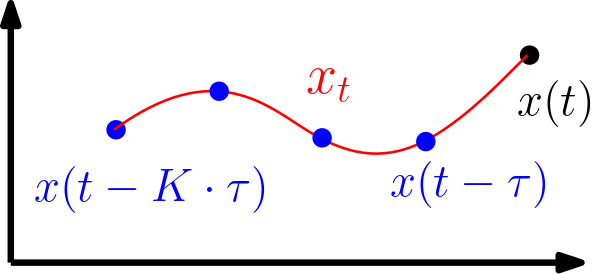
\includegraphics[scale=0.18]{figures/cont_history.png}}} \end{picture} 
\end{frame}

%%%%%%%%%%%%%%%%%%%%%%%%%%%%%%%%%%%%%%%%%%%%%%%%%%%%
% 2 Neural ODEs
%%%%%%%%%%%%%%%%%%%%%%%%%%%%%%%%%%%%%%%%%%%%%%%%%%%%

\begin{frame}[t]
    \frametitle{Neural ODEs \tiny{\normalfont{\emph{(Chen et al., Neural Ordinary Differential Equations, 2019)}}}}
    \textbf{Model:} \hspace{1.7cm}\raisebox{-0.2cm}{\begin{tikzpicture}[minimum size=0.6cm, line width=0.75pt]  
        \node[] (x) {$x(t)$};
        \node[rectangle, draw, right=of x] (nn) {$f_\theta$ NN};
        \node[right=of nn] (dx) {$\dot{x}(t)$};
        \draw[every loop]
        (x) edge[] node {} (nn)
        (nn) edge[] node {} (dx);
    \end{tikzpicture}}\\\vspace{0.2cm}\\
    \textbf{Prediction:} \begin{flalign*}&\hspace{3cm}x(T) = \int_0^T f(x(t),\theta)\,dt +x_0&\end{flalign*}
    
    \textbf{Loss:} \begin{flalign*}&\hspace{3cm}J(\theta) = L(x(T)) + \int_0^T \ell(x(t))\,dt\;\to\; \text{e.g. } J = \sum_{k=1}^N \norm{x(t_k)-x_k^{\text{data}}}_2^2&\end{flalign*}
    \textbf{Loss gradients:} 
    \begin{itemize}
        \item Adjoint method 
        \vspace{-1cm}\begin{figure}\centering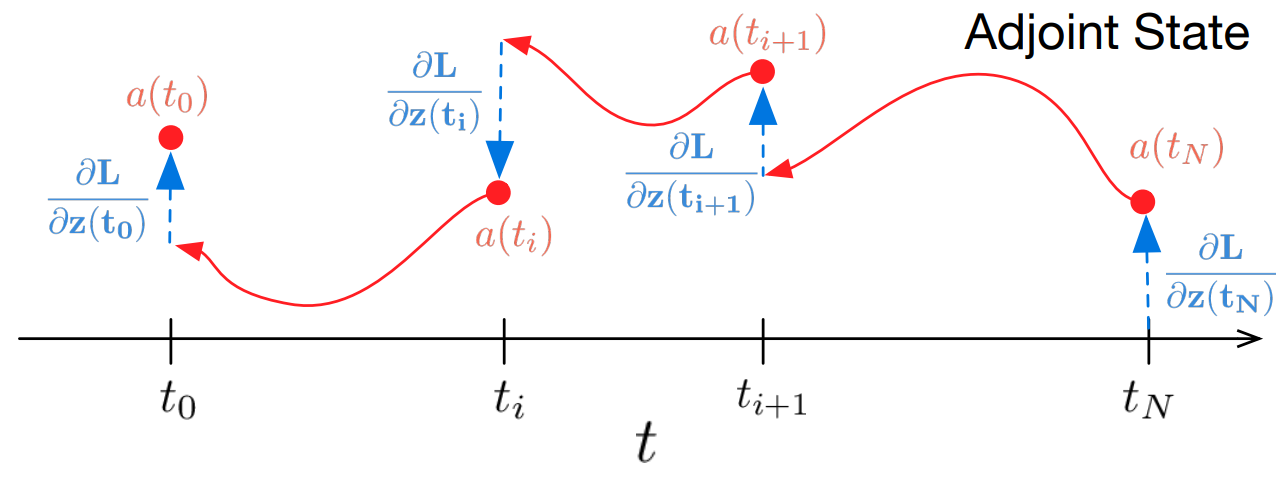
\includegraphics[width=0.4\textwidth]{figures/adjoint.png}\end{figure}
        \item Discrete sensitivities $\to$ automatic differentiation through solver
    \end{itemize}
\end{frame}


%%%%%%%%%%%%%%%%%%%%%%%%%%%%%%%%%%%%%%%%%%%%%%%%%%%%
% 3 Neural NDDEs
%%%%%%%%%%%%%%%%%%%%%%%%%%%%%%%%%%%%%%%%%%%%%%%%%%%%

\begin{frame}[t]
    \frametitle{Neural delay differential equations (NDDE)}
    \textbf{Model:} \hspace{1.7cm}\raisebox{-0.2cm}{\begin{tikzpicture}[minimum size=0.6cm, line width=0.75pt]  
        \node[] (x) {$x(t)$};
        \node[left=0.3cm of x] (x-1) {$x(t-\tau)$};
        \node[left=of x-1] (x-K) {$x(t-K\cdot\tau)$};
        \node[rectangle, draw, right=of x] (nn) {$f_\theta$ NN};
        \node[right=of nn] (dx) {$\dot{x}(t)$};
        \path (x-1) -- node[auto=false]{\ldots} (x-K);
        \draw[every loop]
        (x) edge[] node {} (nn)
        (x-1) edge[bend left] node {} (nn)
        (x-K) edge[bend left] node {} (nn)
        (nn) edge[] node {} (dx);
    \end{tikzpicture}}\\\vspace{0.2cm}\\
    \textbf{Prediction (K=1):} \begin{flalign*}&\hspace{3cm}x(T) = \int_\tau^T f(x(t),x(t-\tau),\theta)\,dt +\int_0^\tau f(x(t),\psi(t-\tau),\theta)\,dt&\end{flalign*}
    
    \textbf{Loss:} \begin{flalign*}&\hspace{3cm}J(\theta) = L(x(T)) + \int_0^T \ell(x(t))\,dt\;\to\; \text{e.g. } J = \sum_{k=1}^N \norm{x(t_k)-x_k^{\text{data}}}_2^2&\end{flalign*}
    \textbf{Loss gradients:} 
    \begin{itemize}
        \item Adjoint method 
        \item Discrete sensitivities $\to$ automatic differentiation through solver
    \end{itemize}
\end{frame}

%%%%%%%%%%%%%%%%%%%%%%%%%%%%%%%%%%%%%%%%%%%%%%%%%%%%
% 5 Partially observed oscillator
%%%%%%%%%%%%%%%%%%%%%%%%%%%%%%%%%%%%%%%%%%%%%%%%%%%%

\begin{frame}[t]
    \frametitle{Partially observed oscillator}
    \textbf{Dynamics:} $\dot{z}(t) = \myvec{0 & 1\\-1 & 0}z(t),\quad y(t) = \myvec{1 & 0}z(t), \quad z(0) =\myvec{1\\0}$
    \begin{columns}[T]
        \begin{column}{0.25\textwidth}
        \pause
            \begin{figure}
                \centering
                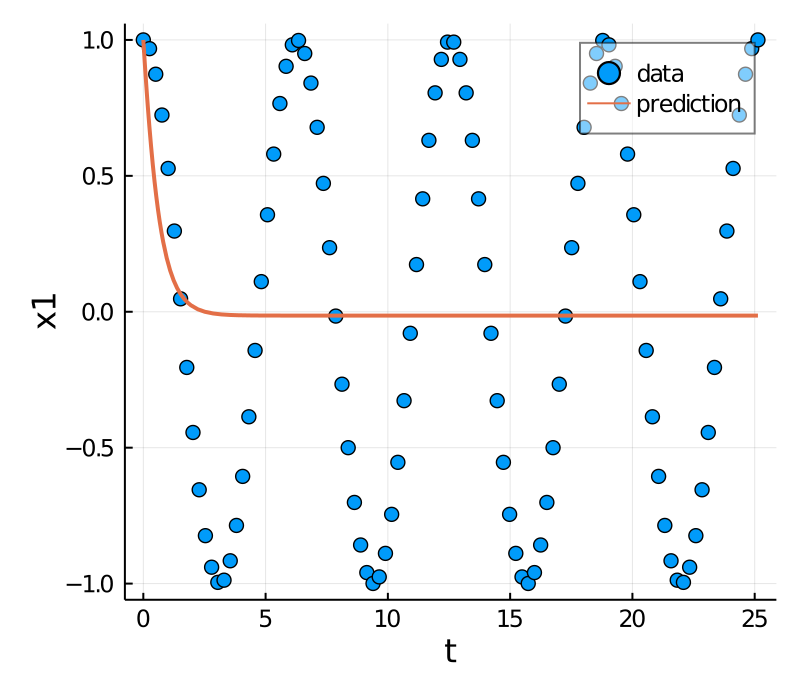
\includegraphics[width=0.94\columnwidth]{figures/vanilla_node.png}
                            \vspace{-0.2cm}
                \caption{Vanilla NODE}
            \end{figure}
        \end{column}
        \begin{column}{0.5\textwidth}
        \onslide<3->{
            \begin{figure}
                \centering
                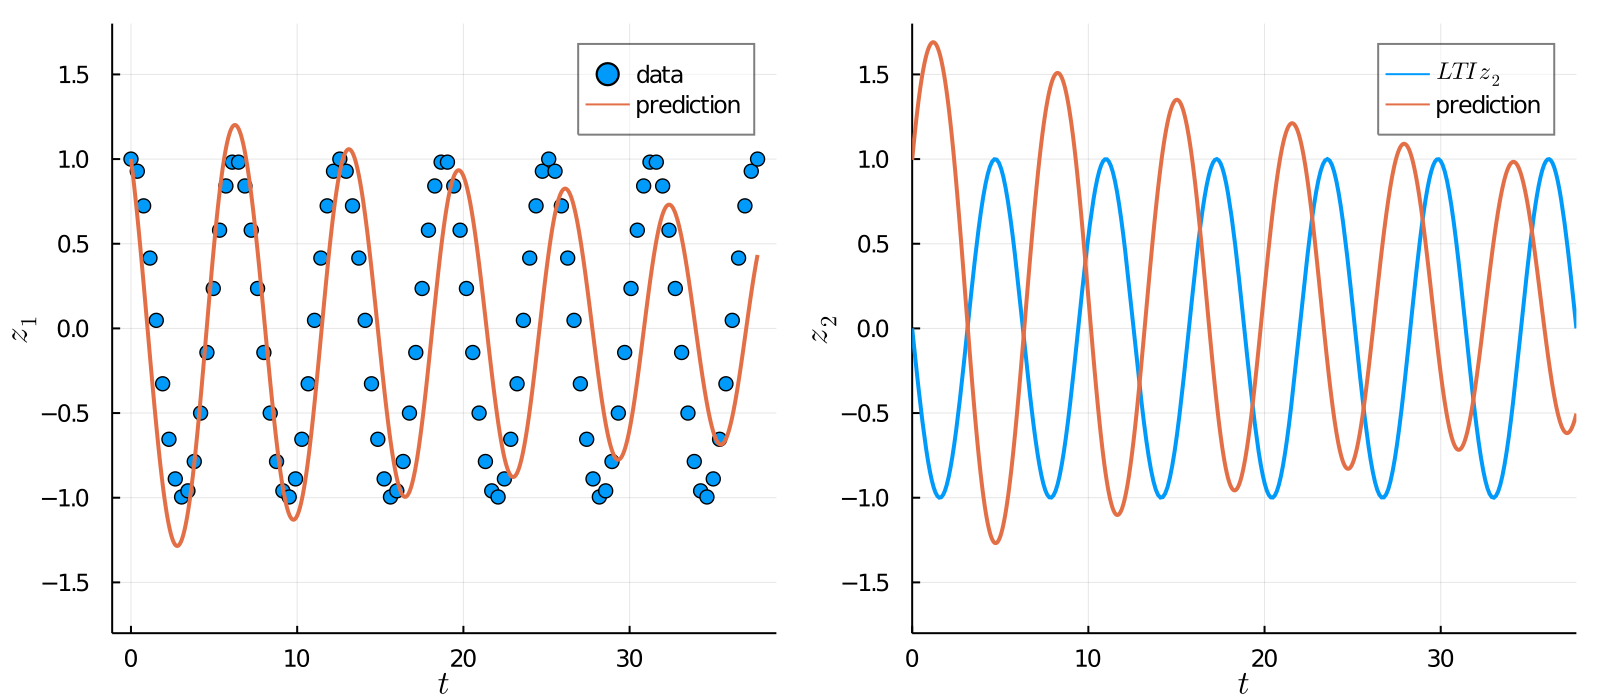
\includegraphics[width=0.9\columnwidth]{figures/anode_learn_init.png}
                                            \vspace{-0.2cm}
                \caption{ANODE learn initial condition}
            \end{figure}}
        \end{column}
        \begin{column}[T]{0.25\textwidth}
        \pause
            \onslide<4->{\begin{figure}
                \centering
                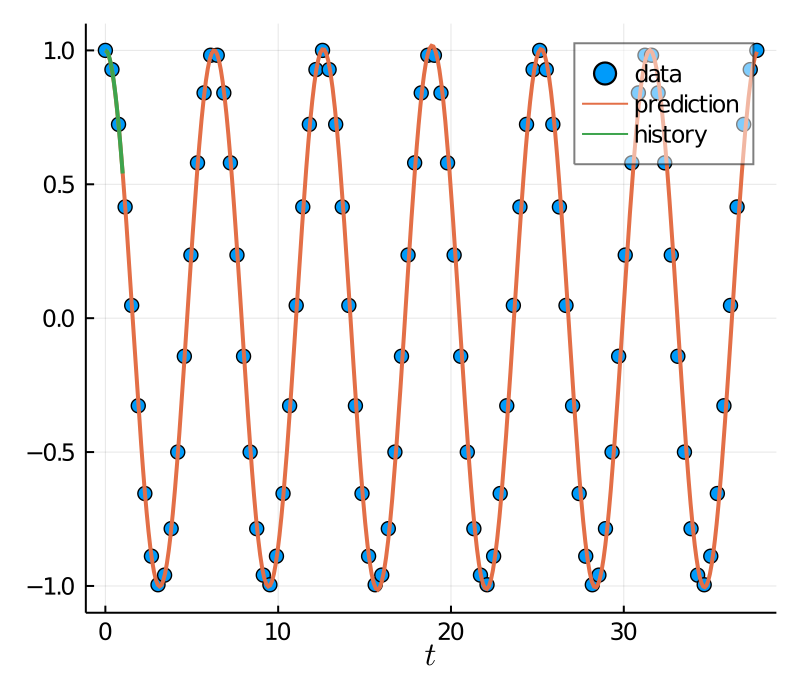
\includegraphics[width=0.94\columnwidth]{figures/ndde.png}                            \vspace{-0.2cm}
                \caption{NDDE $\tau=1, K=1$}
            \end{figure}}
        \end{column}
    \end{columns}
    \vspace{0.2cm}
    \begin{columns}[T]
        \begin{column}[T]{0.5\textwidth}
            \onslide<3->{
            \hspace{0.35cm}\textbf{ANODE:}
            \hspace{0.35cm}\begin{itemize}
                \item Initialization of augmented states problematic
            \end{itemize}}
        \end{column}
        \begin{column}[T]{0.5\textwidth}
            \onslide<4->{\textbf{NDDE:}
            \begin{itemize}
                \item Robustness to observation noise
                \item Generalization over time and initial conditions
                \item Also works on more complex data
            \end{itemize}}
        \end{column}
    \end{columns}

\end{frame}

%%%%%%%%%%%%%%%%%%%%%%%%%%%%%%%%%%%%%%%%%%%%%%%%%%%%
% 4 Expressivity
%%%%%%%%%%%%%%%%%%%%%%%%%%%%%%%%%%%%%%%%%%%%%%%%%%%%

\begin{frame}[t]
    \frametitle{Theoretical insights on expressivity}
    \textbf{Universal approximation theorem for input-output-map}\\\vspace{0.1cm}
    For any $H:\R^n \to\R^n$ there is a DDE with a single delay and input-output-map $\Phi: \psi_{x_0}\mapsto x(T)$ such that for a fixed $T$ it holds $x(0)=x_0$ and $x(T)=H(x_0)$.\\\vspace{0.1cm}
    \begin{tikzpicture}[text height=2ex]
        \node (a) {$x_0$};
        \node (b) [right=1cm of a] {$\psi_{x_0}$};
        \node (c) [rectangle,draw, right=1.2cm of b] {NDDE};
        \node (d) [right=1cm of c] {$x(T)=H(x_0)$};
        \node (e) [text centered,  left=-0.05cm of c] {$\displaystyle\int$};
        \draw[every loop]
        (a) edge[] node {} (b)
        (b) edge[] node {} (e)
        (c) edge[] node {} (d);
    \end{tikzpicture}\\
    \vspace{0.25cm}
    \pause
    \textbf{Approximation along trajectory}
    \begin{itemize}
        \item Can approximate truncated Fourier series as solutions of linear DDEs
        \item Approximation of $1-$dimensional observations of periodic and chaotic attractors (Takens Embedding Theorem)
     \end{itemize}
    \begin{figure}
        \centering
        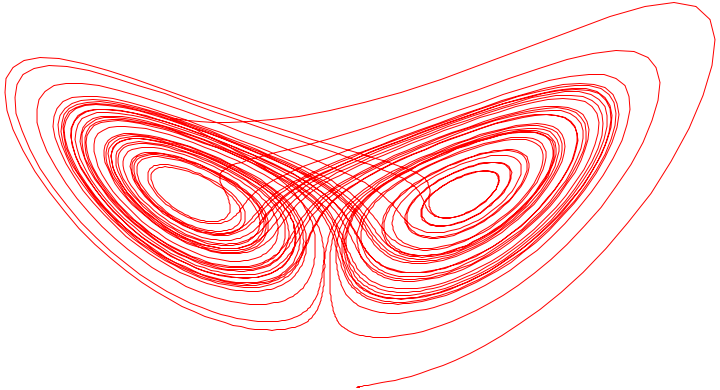
\includegraphics[width=0.4\textwidth]{figures/lorenz.png}
    \end{figure}
\end{frame}

%%%%%%%%%%%%%%%%%%%%%%%%%%%%%%%%%%%%%%%%%%%%%%%%%%%%
% 7 Stability definition
%%%%%%%%%%%%%%%%%%%%%%%%%%%%%%%%%%%%%%%%%%%%%%%%%%%%

\begin{frame}[t]
    \frametitle{Exponential stability of time delay systems}
    \begin{definition}
    The time delay system $\dot{x}(t) = f(x_t)$ is said to be exponentially stable if there exist $M>0, \gamma>0$ such that for any initial history $x_{t_0} = \psi$ it holds,
    $$\norm{x(t)}_2 \leq e^{-\gamma (t-t_0)}M\norm{\psi}_\infty \quad \text{for } t\geq t_0.$$
    \end{definition}
    \textbf{Example: } $\dot{x}(t) = -x(t-\tau) \to$ exponentially stable for $\tau<\pi/2$.
    \begin{figure}
        \centering
        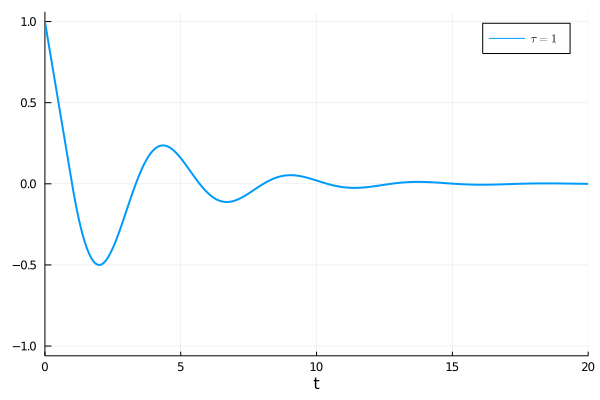
\includegraphics[width=0.35\textwidth]{figures/linear_dde.png}
        \vspace{-0.2cm}
        \caption{$\tau = 1$ and $x(t)=1$ for $t\leq 0$}
    \end{figure}
    
\end{frame}

%%%%%%%%%%%%%%%%%%%%%%%%%%%%%%%%%%%%%%%%%%%%%%%%%%%%
% 8 Stability
%%%%%%%%%%%%%%%%%%%%%%%%%%%%%%%%%%%%%%%%%%%%%%%%%%%%

\begin{frame}[t]
    \frametitle{Non-linear stability analysis \tiny{\normalfont{\emph{(Manek et al., 2020; Richards et al., 2018)}}}}
    \textbf{non-delayed case} \; $\dot{x}(t) = f(x(t))$
        \begin{itemize}
            \item Lyapunov functions (for exponential stability)
                \begin{itemize}
                    \item $c_1\norm{x}_2^p \leq V(x) \leq c_2\norm{x}_2^p$
                    \item $\dot{V}\left(x(t)\right)\leq -\alpha V(x(t))$ \hspace{1.5cm} $\to$ hard to find
                \end{itemize}
            \item ML approach: Learn a neural network Lyapunov function $V_\phi$
        \end{itemize}
        \vspace{0.5cm}
    \textbf{time delay systems} \; $\dot{x}(t) = f(x_t),\; x_t(s)=x(t+s),\; s\in[-r,0]$
        \begin{itemize}
            \item Lyapunov-Krasovskii functionals\\
            $\to$ natural extension of Lyapunov functions to time delay systems
            \item Lyapunov-Razumikhin functions\\
            $\to$ use Lyapunov functions, but relax decay condition
            
        \end{itemize}
\end{frame}

%%%%%%%%%%%%%%%%%%%%%%%%%%%%%%%%%%%%%%%%%%%%%%%%%%%%
% 9 Razumikhin Theorem
%%%%%%%%%%%%%%%%%%%%%%%%%%%%%%%%%%%%%%%%%%%%%%%%%%%%

\begin{frame}[t]
    \frametitle{Lyapunov-Razumikhin functions (exponential stability)} 
    \begin{theorem}[Liu et al, 2012]
    Assume there exists a differentiable function \\$V:\R\times\R^n\to \R_+$ and constants $q>1, c_1>0, c_2>0, \alpha>0$ such that the following hold:
    \begin{enumerate}[(i)]
        \item $c_1 \norm{x}_2^2 \leq V(x) \leq c_2 \norm{x}_2^2$
        \item $\dot{V}(x(t)) \leq -\alpha V(x(t))$\\
        whenever $V(x(t+s))\leq q V(x(t)) \quad\forall s\in [-r,0]$.
    \end{enumerate}
    Then $\dot{x}(t) = f(x_t)$ is exponentially stable with decay rate $\gamma = \min(\alpha, \frac{\log q}{r})/2$.
\end{theorem}
\textbf{Intuition:} Require decay condition only when we are about to leave the sublevel set \;$V^{\leq \eta}$ of \linebreak $\eta := \sup_{s\in [-r,0]} V(x(t+s))$.

\begin{columns}
    \begin{column}{0.5\textwidth}
        \begin{figure}
        \centering
        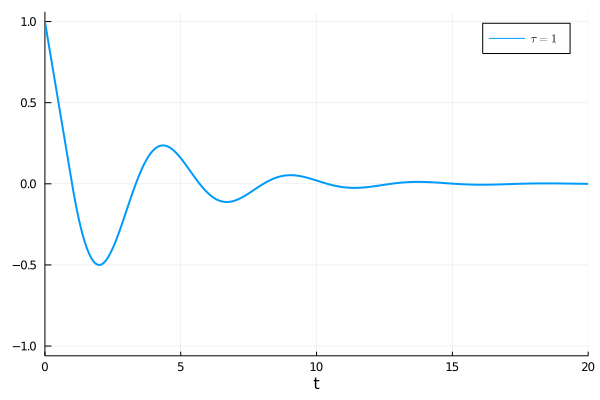
\includegraphics[width=0.5\columnwidth]{figures/linear_dde.png}
        \end{figure}
    \end{column}
        \begin{column}{0.5\textwidth}
        \hspace{-1cm}\begin{figure}
        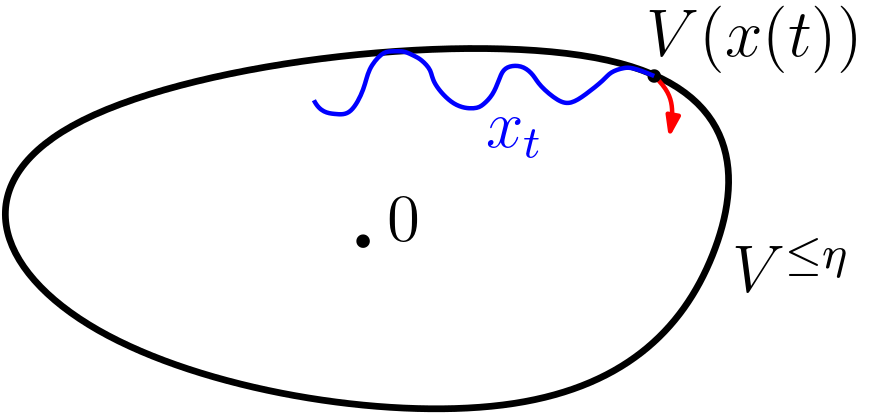
\includegraphics[scale=0.15]{figures/sublevelset.png}
        \end{figure} 
    \end{column}
\end{columns}

\end{frame}

%%%%%%%%%%%%%%%%%%%%%%%%%%%%%%%%%%%%%%%%%%%%%%%%%%%%
% 10 Discretization of Razumikhin Condition
%%%%%%%%%%%%%%%%%%%%%%%%%%%%%%%%%%%%%%%%%%%%%%%%%%%%

\begin{frame}[t]
\frametitle{Discretization of Razumikhin Condition}
We need $\dot{V}(x(t_0)) \leq -\alpha V(x(t_0))$ whenever...
\begin{itemize}
    \item \only<1>{$V(x(t_0+s))\leq q V(x(t_0)), \quad\forall s\in [-r,0]$}\only<2->{\redout{$V(x(t_0+s))\leq q V(x(t_0)), \quad\forall s\in [-r,0]$}}\\
    \pause
    \item<2-> $V(x(t_0-k\tau))\leq q V(x(t_0)) \quad,\forall k\in \lbrace 0,1,...,K\rbrace$
\end{itemize}
\pause
\vspace{0.3cm}
\textbf{Want: }\\\vspace{-0.6cm}
\begin{align*}
    V(x(t_0-k\tau))&\leq q V(x(t_0)) \quad,\forall k\in \lbrace 0,1,...,K \rbrace&\\
    &\big\Downarrow\\
    V(x(t_0+s))&\leq \tilde{q}(\tau)V(x(t_0)), \quad\forall s\in [-r,0], \text{ with } \tilde{q}(\tau)= q+\mathcal{O}(\tau^2) \text{ as } \tau\to 0.
\end{align*}
\pause\vspace{0.}
\textbf{Assumptions:}
Some technical assumptions $+$ either of the following:
\begin{itemize}
    \item  $\max_{s\in[t_0-r_V,t_0]} \norm{x(s)}_2 \geq \varepsilon$\\\vspace{0.1cm}
    \textcolor{red}{$\to$ show convergence to $\varepsilon-$neighbourhood of origin only}\vspace{0.1cm}
    \item $\max_{s\in[t_0-r_V,t_0]} \norm{x(s)}_2 \leq g(c)\max_{s\in[t_0-r_V+c,t_0+c]}\norm{x(s)}_2$ \\\vspace{0.1cm}
    \textcolor{red}{$\to$ satisfied for exponentially decaying oscillations (if $r_V$ large enough)}
\end{itemize}
\end{frame}

%%%%%%%%%%%%%%%%%%%%%%%%%%%%%%%%%%%%%%%%%%%%%%%%%%%%
% 11 Soft-stability enforcement
%%%%%%%%%%%%%%%%%%%%%%%%%%%%%%%%%%%%%%%%%%%%%%%%%%%%

\begin{frame}[t]
    \frametitle{Soft-stability enforcement}
    \textbf{Goal:} Jointly learn $\dot{x}(t) = f_\theta(x(t),...,x(t-K\cdot\tau))$ and a NN $V_\phi$ such that:
    \begin{equation*}
        \dot{V}(x(t_0)) \leq -\alpha V(x(t_0)) \text{ whenever } V(x(t_0-k\tau))\leq q V(x(t_0)) \quad,\forall k\in \lbrace 0,1,...,K\rbrace
    \end{equation*}
    \pause\vspace{0.2cm}
    \textbf{Add loss:}
    \begin{tcolorbox}[ams align*, colframe=red]
\ell\left(\V{x_\tau}(t)\right) = \text{ReLU}\left(\dot{V}_{\phi,\theta}\left(\V{x_\tau}(t)\right)+\alpha V_\phi(x(t))\right) R_\phi\left(\V{x_\tau}(t)\right)
\end{tcolorbox}
    \begin{itemize}
        \item $\V{x_\tau}(t) = \myvec{x(t),x(t-\tau),...,x(t-K\cdot\tau)}$
        \item $R_\phi(\V{x_\tau}(t)) := \prod_{k=1}^K \Theta\left(q V(x(t))-V(x(t-k\cdot\tau))\right)$, \; $\Theta$ unit step function
        \item $V_\phi(x(t))$ based on input convex neural network
    \end{itemize}
    \vspace{0.2cm}
    $\to$ If $\ell\left(\V{x_\tau}(t)\right)$ is zero along a trajectory, then this trajectory converges exponentially towards\\ \hspace{0.45cm}the origin.
    
\end{frame}

%%%%%%%%%%%%%%%%%%%%%%%%%%%%%%%%%%%%%%%%%%%%%%%%%%%%
% 12 Training
%%%%%%%%%%%%%%%%%%%%%%%%%%%%%%%%%%%%%%%%%%%%%%%%%%%%

\begin{frame}[t]
    \frametitle{Training}
    \textbf{Along trajectory}\\
        Minimize continuous loss along solution.\vspace{0.2cm}
        \begin{flalign*}
            J(\phi,\theta) &= \int_0^T \ell_d\left(\V{x_\tau}(t)\right) dt\\
            &= \int_0^T \textcolor{red}{\sigma_d}\left(\dot{V}_{\phi,\theta}\left(\V{x_\tau}(t)\right)+\alpha V_\phi(x(t))\right) \prod_{k=1}^K \textcolor{red}{\Theta_d}\left(q V(x(t))-V(x(t-k\cdot\tau))\right)dt& 
        \end{flalign*}
        $\to$ need \textcolor{red}{smoothed step} and \textcolor{red}{ReLU} for DDE solver. Theoretically sound!\\
    \vspace{0.4cm}
    \only<2->{
    \textbf{Uncorrelated}\\
    Create data set $\lbrace \V{x}^{(i)} \rbrace_{i=1}^N$ of samples $ \V{x}^{(i)}\in \R^{n(K+1)}$ and minimize $\frac{1}{N}\sum_{i=1}^N \ell\left(\V{x}^{(i)}\right)$.\\
    \vspace{0.25cm}
    $\to$ no need for smoothing, but more conservative\\}
    \only<1>{\begin{picture}(50,50) \put(250,115){\hbox{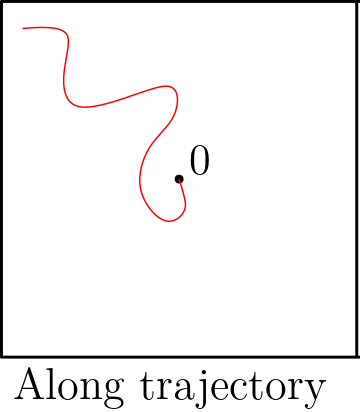
\includegraphics[scale=0.275]{figures/stab_training_traj.png}}}
    \end{picture}}\only<2->{\begin{picture}(50,50) \put(250,150){\hbox{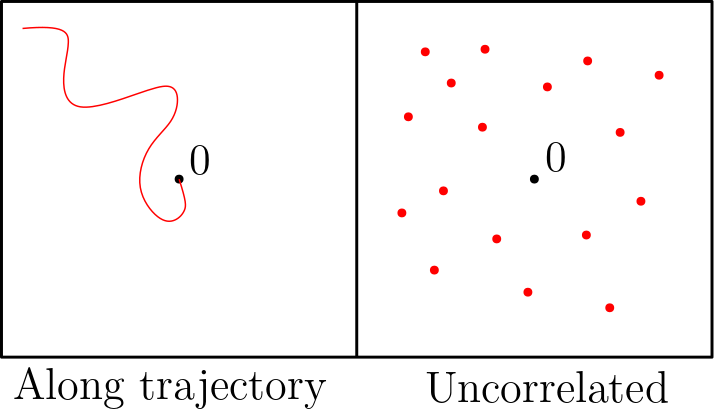
\includegraphics[scale=0.2]{figures/stab_training.png}}}
    \end{picture}}
\end{frame}

%%%%%%%%%%%%%%%%%%%%%%%%%%%%%%%%%%%%%%%%%%%%%%%%%%%%
% 13 Application
%%%%%%%%%%%%%%%%%%%%%%%%%%%%%%%%%%%%%%%%%%%%%%%%%%%%

\begin{frame}[t]
    \frametitle{Application}
    \textbf{Inverted pendulum with delayed feedback} \emph{(Milton et al., 2009)}\quad $x(t)=\left(\varphi(t), \dot{\varphi}(t)\right)^\top$    
    \vspace{0.2cm}
    \begin{flalign*}
        &\dot{x}(t) = \myvec{\dot{x_1}(t)\\\dot{x_2}(t)} = \myvec{x_2(t)\\\dfrac{g}{l} \sin(x_1(t)) - \dfrac{b}{ml^2}x_2(t) + \dfrac{1}{ml^2}u(t-\tau)}&    
    \end{flalign*}
    
    \pause
    \vspace{0.5cm}\hspace{-0.1cm}
    \only<1->{\textbf{Policy:} $u(t) = \pi(x(t)) = k_1 x_1(t) + k_2 x_2(t) \;\to$ initialized with LQR}\\
    \vspace{0.5cm}
    \only<1->{\textbf{Goal:} Learn linear stabilizing $k_1,k_2$ and $V_\phi$\\
    \vspace{0.5cm}
    \begin{columns}[T]
        \begin{column}[T]{0.5\textwidth}
            \hspace{0.35cm}\textbf{Along trajectory:}
            \begin{itemize}
                \item Time horizon $T=1.5$
                \item Initial position $x_0=(0,-0.5)^\top$
            \end{itemize}
        \end{column}
        \begin{column}[T]{0.5\textwidth}
            \textbf{Uncorrelated:}
            \begin{itemize}
                \item $\V{x}^{(i)}\sim \mathcal{U}([-\pi/2,\pi/2]^{2(K_V+2))}$\\
                \vspace{0.2cm}
                \begin{tabular}{ c |c  }
                    data size & batch size\\                    
                    \hline
                    64'000 & 64
                \end{tabular}
            \end{itemize}
        \end{column}
    \end{columns}}
\only<1->{\begin{picture}(50,50) \put(285,110){\hbox{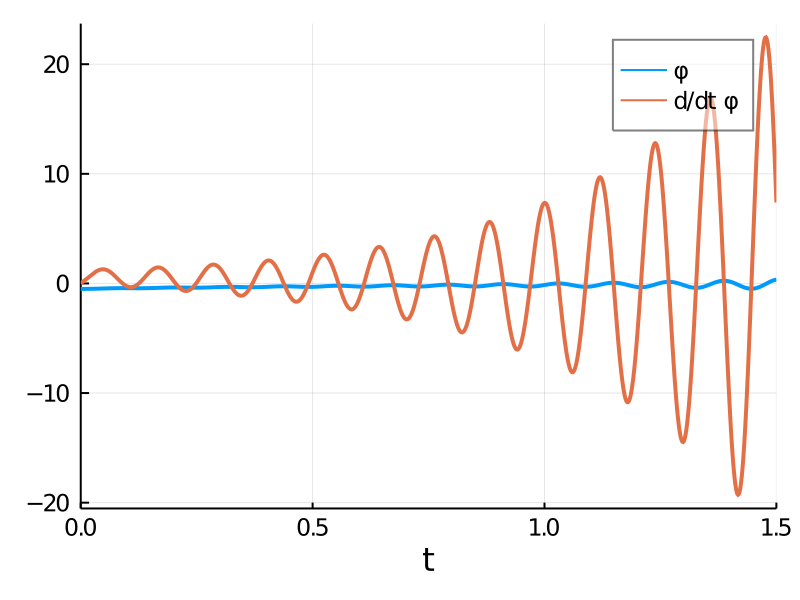
\includegraphics[scale=0.15]{figures/LQR.png}}}
\end{picture}}
\end{frame}


%%%%%%%%%%%%%%%%%%%%%%%%%%%%%%%%%%%%%%%%%%%%%%%%%%%%
% 14 Stabilization experiments
%%%%%%%%%%%%%%%%%%%%%%%%%%%%%%%%%%%%%%%%%%%%%%%%%%%%

\begin{frame}
    \frametitle{Stabilization experiments}
    \begin{columns}[T]
        \begin{column}{0.3\textwidth}
            \vspace{-1cm}
            \begin{figure}[h!]
                 \centering
                 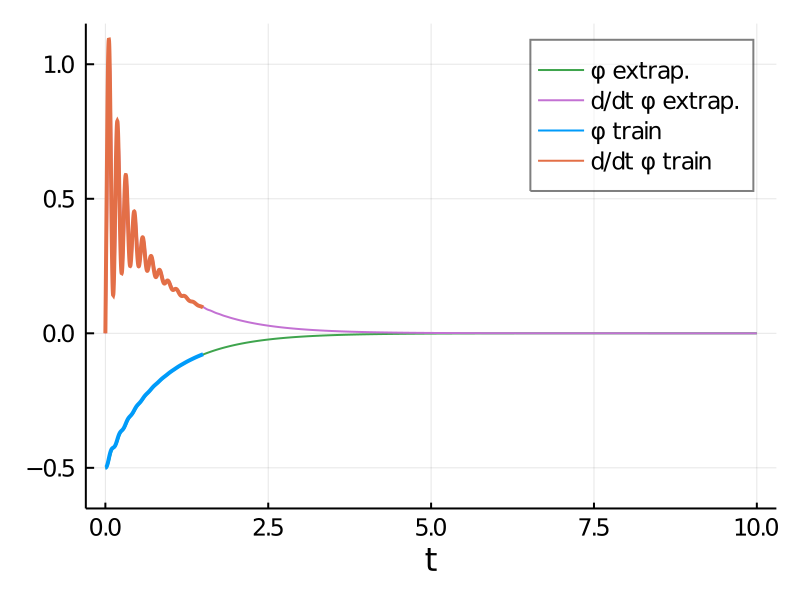
\includegraphics[width=\columnwidth]{figures/nn_cont/extrapolation10.png}
             \end{figure}
             \vspace{-1cm}
             \begin{figure}[h!]
                 \centering
                 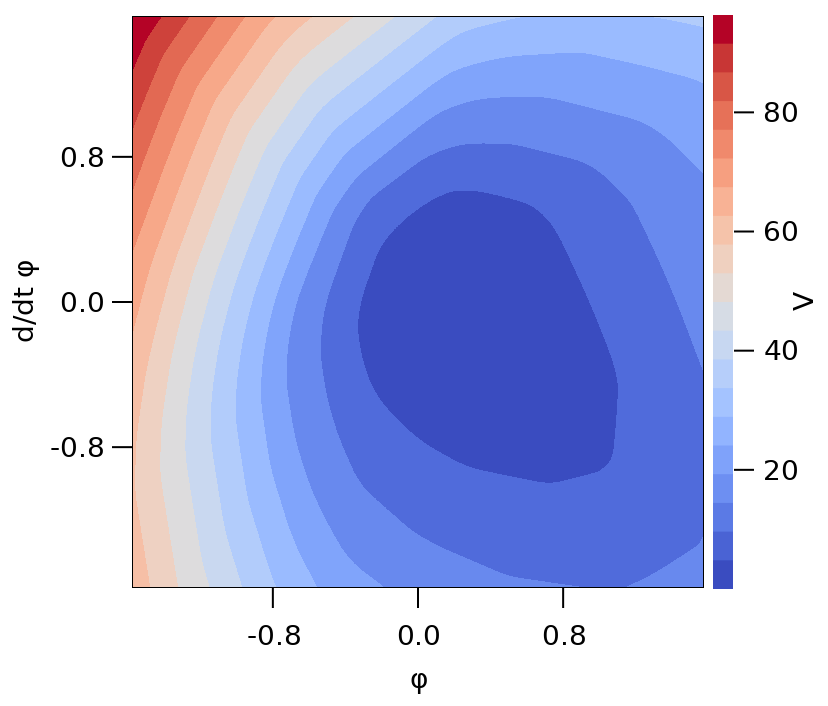
\includegraphics[width=\columnwidth]{figures/nn_cont/V_trained.png}
                 \vspace{-0.5cm}
                 \caption{Along single trajectory}
             \end{figure}
        \end{column}
        \begin{column}{0.3\textwidth}
        \vspace{-1cm}
            \begin{figure}[h!]
                \centering
                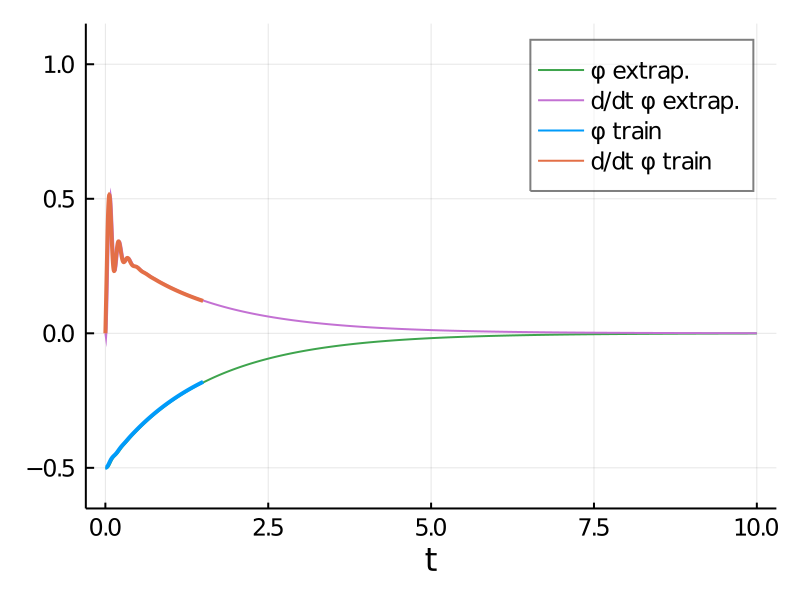
\includegraphics[width=\columnwidth]{figures/nn_disc/extrapolation10.png}
            \end{figure}
            \vspace{-1cm}
            \begin{figure}[h!]
                 \centering
                 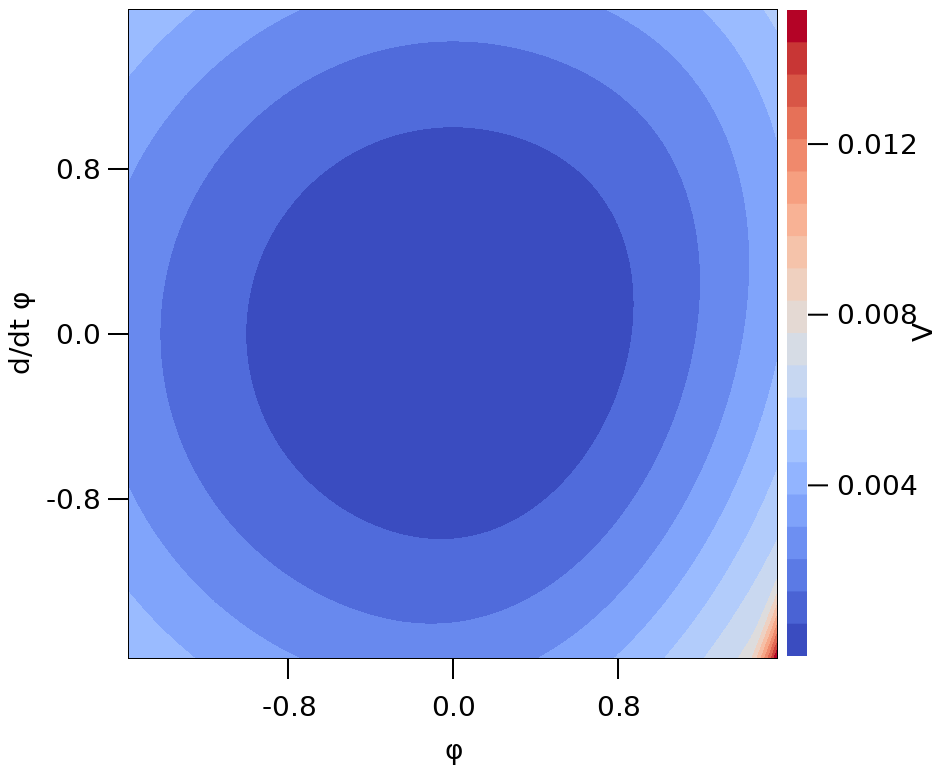
\includegraphics[width=\columnwidth]{figures/nn_disc/V_nn_trained_uncorrelated.png}
                 \caption{Uncorrelated}
             \end{figure}
        \end{column}
        \begin{column}[T]{0.4\textwidth}
        \textbf{Generalization}\\
        Evaluate continuous loss along 8 trajectories starting from
        $x(0)=(\cos(2\pi l/8), \sin(2\pi l/8))_{l=1}^8$
            \begin{center}
                \begin{tabular}{ l | c }
 method& test loss\\
 \hline
  along trajectory& 3.1502\\
  uncorrelated& 0.0000\\
  LQR& unstable
\end{tabular}
            \end{center}
        \end{column}
    \end{columns}
\end{frame}

\begin{frame}[t]
    \frametitle{Conclusion}
    \textbf{Summary:}
    \begin{itemize}
        \item Introduced neural DDEs
        \item Modelling partially observed dynamical systems
        \item Theoretical results on expressivity of neural DDEs
        \item Learning Lyapunov-Razumikhin functions
        \item Stabilization of inverted pendulum with delayed feedback control
    
    \end{itemize}
    \vspace{0.3cm}
    \textbf{Outlook:}
    \begin{itemize}
        \item More complicated systems
        \item Global stability guarantees
    \end{itemize}
\end{frame}

\begin{closingframe}
  \centering \Large
  Thank you :)
\end{closingframe}

%%%%%%%%%%%%%%%%%%%%%%%%%%%%%%%%%%%%%%%%%%%%%%%%%%%%
%%%%%%%%%%%%%%%%%%%%%%%%%%%%%%%%%%%%%%%%%%%%%%%%%%%%
% Bonus slides:

%%%%%%%%%%%%%%%%%%%%%%%%%%%%%%%%%%%%%%%%%%%%%%%%%%%%
% B1 Discretization of Razumikhin Condition
%%%%%%%%%%%%%%%%%%%%%%%%%%%%%%%%%%%%%%%%%%%%%%%%%%%%

\begin{frame}[t]
    \frametitle{Discretization of Razumikhin Condition} 
Let $K$ and $\tau$ be such that $r_V:=K\tau\geq r$ and let $x(\cdot)$ be a solution of $\dot{x}(t)=f(x_t)$ passing through $x_{t_0}\in\mathcal{C}([-r,0])$. Let $\rho:=\max_{s\in[t_0-r_V,t_0]} \norm{x(s)}_2<\infty$ and assume $f$ to be $L_f$-Lipschitz with respect to $\norm{\cdot}_\infty$. Moreover, let $V:\R^n\to\R_+$ be convex with,
$$c_1 \norm{x}_2^2 \leq V(x) \leq c_2 \norm{x}_2^2,$$
$f$ and $V$ both be differentiable, and assume that there is a function $g:\R_+\to\R_+$ with $g(s)\geq 1$ such that along the trajectory it holds for any $t$ and $c>0$,
\begin{equation}
    \max_{s\in[t-r_V,t]} \norm{x(s)}_2 \leq g(c) \max_{s\in[t-r_V+c,t+c]}\norm{x(s)}_2.\label{eq:small_decay_cond}
\end{equation}
Now if,
\begin{equation}
    V(x(t_0-k\tau))\leq q V(x(t_0)) \quad,\forall k\in \lbrace 0,1,...,K \rbrace,\label{eq:DiscRazConProp}
\end{equation}
and $8c_1 > (4c_2-c_1)L_f^2 g(2r) \tau^2$, then it holds for any $s\in[-r_V,0]$,
\begin{align}
    V(x(t_0+s))&\leq \tilde{q}(\tau)V(x(t_0)),\label{eq:ContRazConProp}\\
    \text{with } \tilde{q}(\tau)&= \dfrac{q}{1-(4c_2-c_1)L_f^2g(2r)\tau^2/(8c_1)}=q+\mathcal{O}(\tau^2).\nonumber
\end{align}
\end{frame}


%%%%%%%%%%%%%%%%%%%%%%%%%%%%%%%%%%%%%%%%%%%%%%%%%%%%
% B2 Noisy observations
%%%%%%%%%%%%%%%%%%%%%%%%%%%%%%%%%%%%%%%%%%%%%%%%%%%%

\begin{frame}
    \frametitle{Noisy observations}
    \begin{columns}
        \begin{column}{0.5\textwidth}
            \begin{figure}[h!]
                 \centering
                 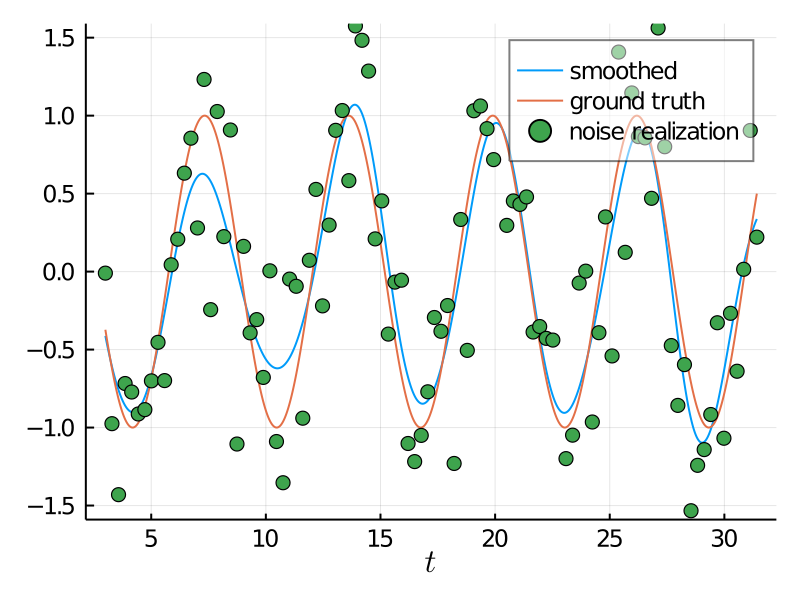
\includegraphics[width=\columnwidth]{figures/10d05sigma_smoothed.png}
                 \caption{Noise $\sigma=0.5$}
             \end{figure}
        \end{column}
        \begin{column}{0.5\textwidth}
            \begin{figure}[h!]
                \centering
                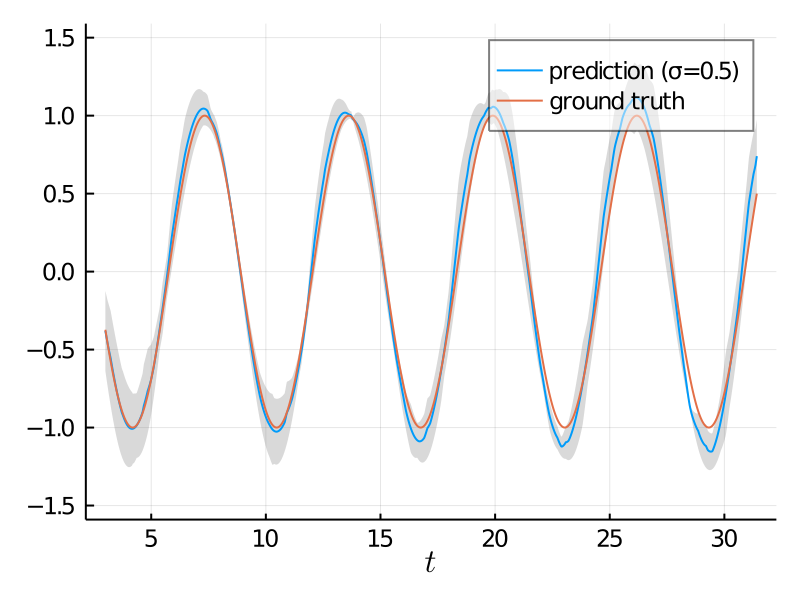
\includegraphics[width=\columnwidth]{figures/10d05sigma_conf.png}
                \caption{$K=10, \sigma=0.5$}
            \end{figure}
        \end{column}
    \end{columns}
\end{frame}


%%%%%%%%%%%%%%%%%%%%%%%%%%%%%%%%%%%%%%%%%%%%%%%%%%%%
% B3 Partially observed oscillator -> delete this
%%%%%%%%%%%%%%%%%%%%%%%%%%%%%%%%%%%%%%%%%%%%%%%%%%%%

\begin{frame}[t]
    \frametitle{Partially observed oscillator $\ddot{x}(t) + x(t) = 0, x(0)=1, \dot{x}(0) = 0$}
    \begin{columns}
        \begin{column}{0.25\textwidth}
            \begin{figure}
                \centering
                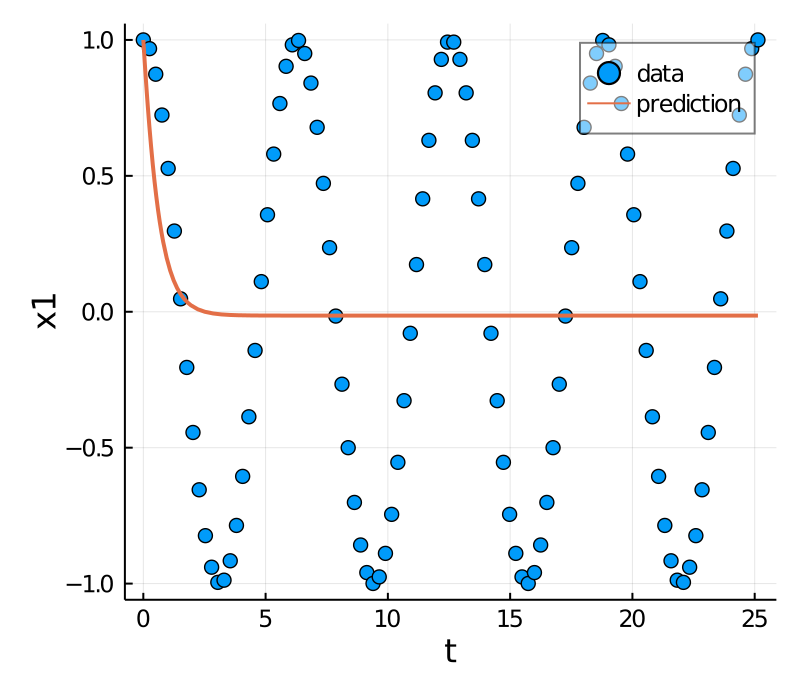
\includegraphics[width=\columnwidth]{figures/vanilla_node.png}
                \caption{Vanilla NODE}
            \end{figure}
        \end{column}
        \begin{column}{0.5\textwidth}
            \vspace{-0.3cm}
            \begin{figure}
                \centering
                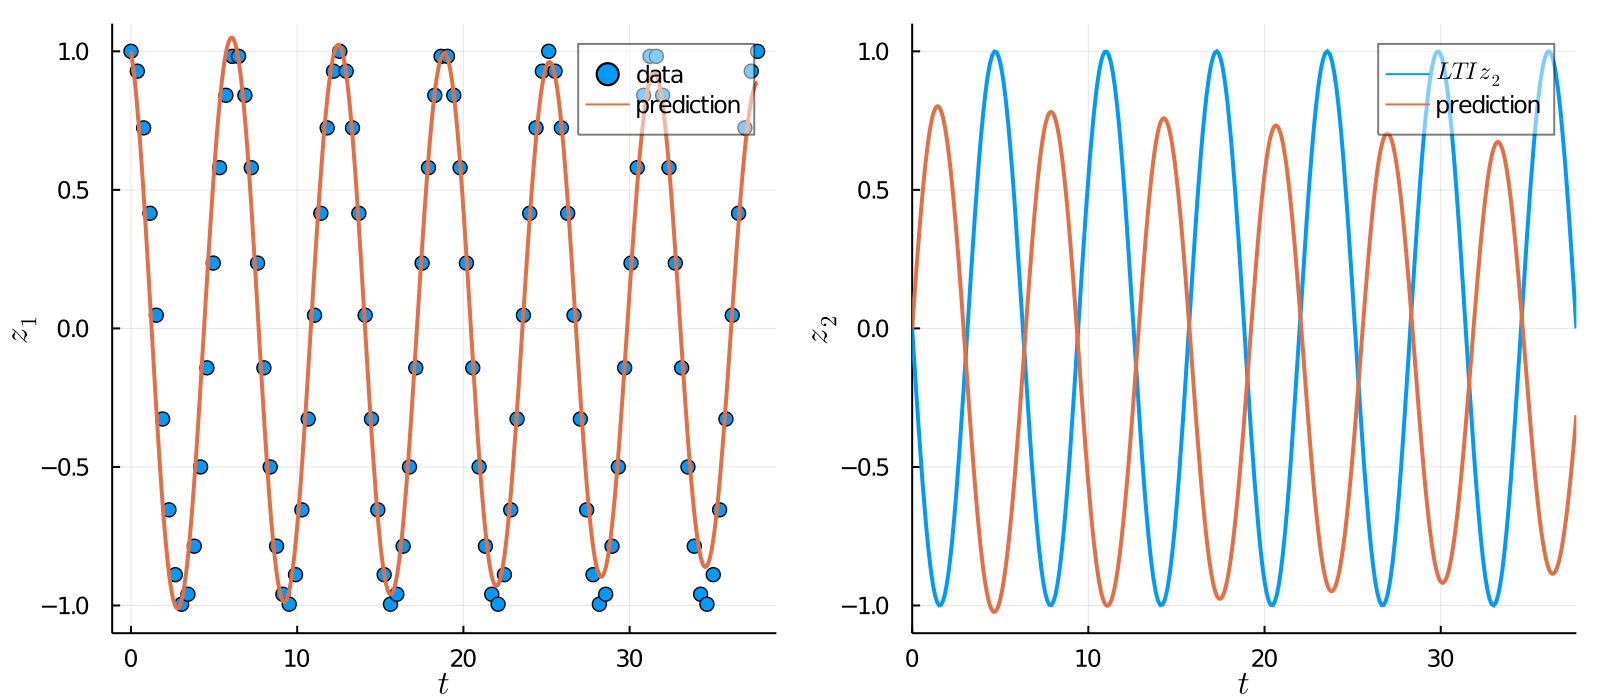
\includegraphics[width=0.9\columnwidth]{figures/anode_true_init.png}
                \caption{ANODE true initial condition}
            \end{figure}
            \vspace{-0.7cm}
            \begin{figure}
                \centering
                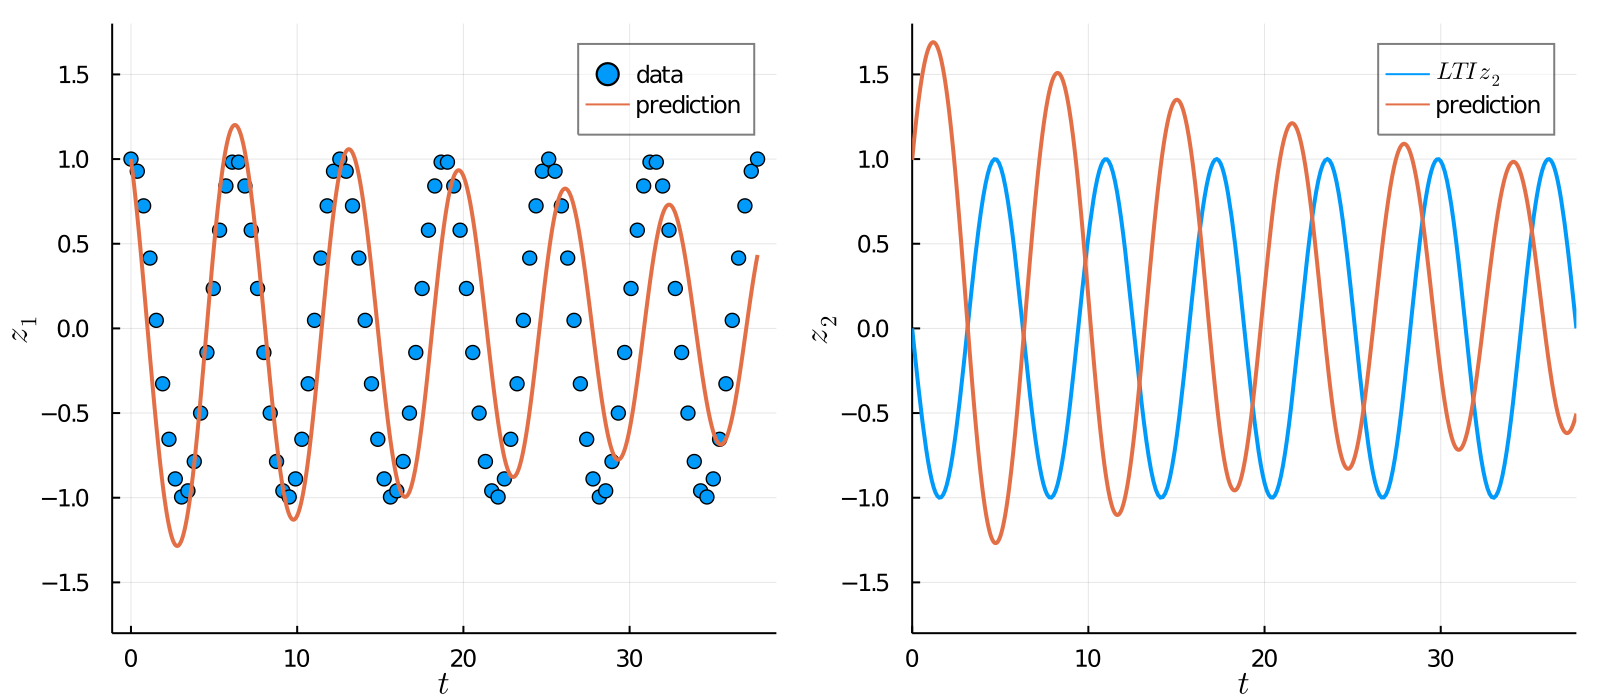
\includegraphics[width=0.9\columnwidth]{figures/anode_learn_init.png}
                \caption{ANODE learn initial condition}
            \end{figure}
        \end{column}
        \begin{column}{0.25\textwidth}
            \begin{figure}
                \centering
                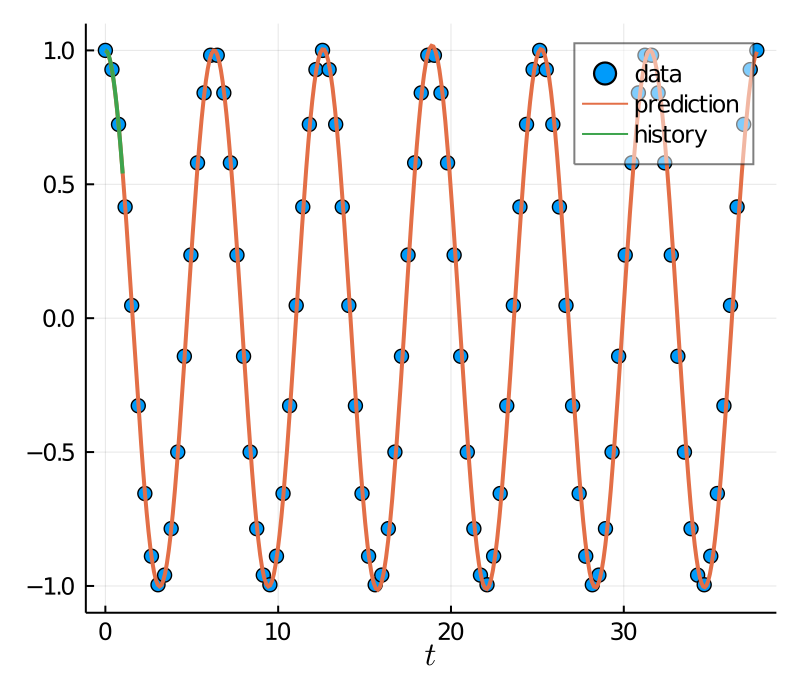
\includegraphics[width=\columnwidth]{figures/ndde.png}
                \caption{NDDE}
            \end{figure}
        \end{column}
    \end{columns}
\end{frame}


\begin{frame}{Pendelum setup}
        \textbf{Pendulum Setup}\vspace{-0.5cm}
    \begin{center}\begin{tabular}{  c | c | c | c |c  }
          $l$ & $m$ & $b$ & $g$ & $\tau$ \\
         \hline
           0.3 & 0.2 & 0 & 9.81 &0.03
        \end{tabular}\end{center}
    \begin{tabular}{ l | c | c | c | c |c | c |c |c| c  }
     training & $\tau_V$ & $K_V$& $r_V $  & $\alpha$ & $q$ &$T$ & $d_L$ & data size & batch size\\
     \hline
      along trajectory& 0.04 & 5 & 0.2 & 0.1 & 1.0202 & 1.5& 0.5& - & - \\
      uncorrelated& 0.04 & 5 & 0.2 & 0.1 & 1.0202 & - & - & 64000 & 64
    \end{tabular}
\end{frame}
\end{document}